\documentclass{amsart}
\usepackage{enumerate}
\usepackage{amsmath}
\usepackage{scrextend}
\usepackage{graphicx}
\usepackage{enumitem}
\usepackage{tcolorbox}
\usepackage[headheight=12pt,textwidth=7in,top=1in, bottom=1in]{geometry}
\usepackage{listings}
\usepackage{color} %red, green, blue, yellow, cyan, magenta, black, white
\definecolor{mygreen}{RGB}{28,172,0} % color values Red, Green, Blue
\definecolor{mylilas}{RGB}{170,55,241}

%some custom commands you may find useful
\usepackage{xparse}
\DeclareDocumentCommand{\diff}{O{} m}{
	\frac{\mathrm{d} #1}{\mathrm{d}#2}
}
\DeclareDocumentCommand{\difftwo}{O{} m}{
	\frac{\mathrm{d}^2 #1}{\mathrm{d}#2^2}
}
\DeclareDocumentCommand{\pdiff}{O{} m}{
	\frac{\partial #1}{\partial #2}
}
\DeclareDocumentCommand{\pdifftwo}{O{} m}{
	\frac{\partial^{2} #1}{\partial #2^{2}}
}
\DeclareDocumentCommand{\integral}{O{} O{} m O{x}}{
	\int_{#1}^{#2} #3\ \mathrm{d}#4
}
\DeclareDocumentCommand{\sp}{}{
	\qquad \qquad \qquad }{
}
\NewDocumentEnvironment{solution}{}{
	\begin{addmargin}[2em]{0pt}
	}{\end{addmargin} \vskip0.25cm
}

\newenvironment{sysmatrix}[1]
{\left(\begin{array}{@{}#1@{}}}
	{\end{array}\right)}
\newcommand{\ro}[1]{%
	\xrightarrow{\mathmakebox[\rowidth]{#1}}%
}
\newlength{\rowidth}% row operation width
\AtBeginDocument{\setlength{\rowidth}{3em}}

\def\name{Ben Wilfong} %your name goes here
\def\CM{570} %your cm goes here

%these packages create the footer and page numbering
\usepackage{fancyhdr}
\usepackage{lastpage}
\pagestyle{fancy}
\lhead{\name}
%%%%%%%%%%%%%%%%%%%%%%%%%%%%%%%%
\chead{ME 422: Homework Set \#13}
%%%%%%%%%%%%%%%%%%%%%%%%%%%%%%%%
\rhead{CM \CM}
\fancyfoot[C]{\footnotesize Page \thepage\ of \pageref{LastPage}}
\fancypagestyle{firststyle}
{ \renewcommand{\headrulewidth}{0pt}%
	\fancyhf{}%
	\fancyfoot[C]{\footnotesize Page \thepage\ of \pageref{LastPage}}
}


\lstset{language=Matlab,%
	%basicstyle=\color{red},
	breaklines=true,%
	morekeywords={matlab2tikz},
	keywordstyle=\color{blue},%
	morekeywords=[2]{1}, keywordstyle=[2]{\color{black}},
	identifierstyle=\color{black},%
	stringstyle=\color{mylilas},
	commentstyle=\color{mygreen},%
	showstringspaces=false,%without this there will be a symbol in the places where there is a space
	numbers=left,%
	numberstyle={\tiny \color{black}},% size of the numbers
	numbersep=9pt, % this defines how far the numbers are from the text
	emph=[1]{for,end,break},emphstyle=[1]\color{red}, %some words to emphasise
	%emph=[2]{word1,word2}, emphstyle=[2]{style},    
}

\begin{document}
	\noindent
	\thispagestyle{firststyle}
	\begin{tabular}{l}
		{\LARGE \textbf{ME422: Finite Elements 1} }\\
		%%%%%%%%%%%%%%%%%%%%%%%%%
		{\Large Homework Set \#1}
		%%%%%%%%%%%%%%%%%%%%%%%%%
	\end{tabular} \hfill \begin{tabular}{r}
		\name \\
		CM \CM
	\end{tabular}
	\noindent\makebox[\linewidth]{\rule{\textwidth}{1pt}} \\~\\
	The point types are:
	\begin{figure}[h]
		\centering
		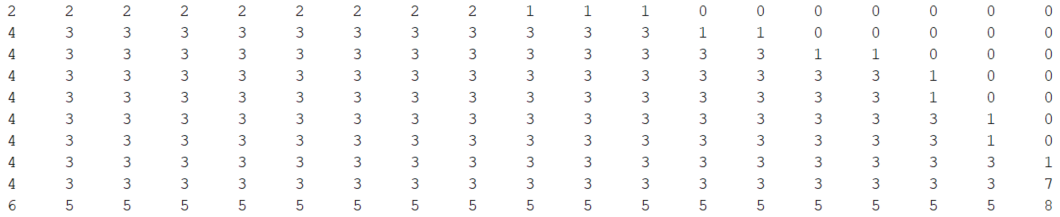
\includegraphics[width=\textwidth]{pointTypes.png}
	\end{figure} \\
	The boundary condition on the curved edge is
	\[\nabla T(x,y,t)\cdot n = -1 \quad \rightarrow \quad \pdiff[T(x,y,t)]{x}n_x + \pdiff[T(x,y,t)]{y}n_y = -1 \quad \rightarrow \quad \pdiff[T_{j,k,i}]{x}n_x + \pdiff[T_{j,k,i}]{y}n_y = -1\]
	At points of type 1 using one sided differences this is:
	\[\frac{n_x}{2h}\left(T_{j,k-2,i} - 4T_{j,k-1,i} + 3T_{j,k,i}\right) + \frac{n_y}{2h}\left(-3T_{j,k,i} + 4T_{j+1,k,i} - T_{j+2,k,i}\right) = -1\]
	\[\frac{3n_x}{2h}T_{j,k,i} - \frac{3n_y}{2h}T_{j,k,i} = -1 + \frac{n_x}{2h}(4T_{j,k-1,i} - T_{j,k-2,i}) + \frac{n_y}{2h}(T_{j+2,k,i} - 4_{j+1,k,i})\]
	\[T_{j,k,i} = \left(\frac{3n_x-3n_y}{2h}\right)^{-1}\left(-1 + \frac{n_x}{2h}(4T_{j,k-1,i} - T_{j,k-2,i}) + \frac{n_y}{2h}(T_{j+2,k,i} - 4_{j+1,k,i})\right)\]
	\noindent At points of type 7 using one sided differences this is:
	\[\frac{n_x}{2h}\left(T_{j,k-2,i} - 4T_{j,k-1,i} + 3T_{j,k,i}\right) + \frac{n_y}{2h}\left(-4T_{j,k,i} + 4T_{j+1,k,i}\right) = -1\]
	\[\frac{3n_x}{2h}T_{j,k,i} - \frac{4n_y}{2h}T_{j,k,i} = -1 + \frac{n_x}{2h}(4T_{j,k-1,i} - T_{j,k-2,i}) - \frac{n_y}{2h}T_{j+1,k,i}\]
	\[T_{j,k,i} = \left(\frac{3n_x-4n_y}{2h}\right)^{-1}\left(-1 + \frac{n_x}{2h}(4T_{j,k-1,i} - T_{j,k-2,i}) - \frac{n_y}{2h}T_{j+1,k,i}\right)\]
	\noindent At points of type 8 using one sided differences this is:
	\[\frac{n_x}{2h}\left(T_{j,k-2,i} - 4T_{j,k-1,i} + 3T_{j,k,i}\right) = -1\]
	\[T_{j,k,i} = -\frac{2h}{n_x} + 4T_{j,k-1,i} - T_{j,k-2,i} \] \newpage
	%%%%%%%%%%%%%%%%%%%%%%%%%%%%%%%%%%%%%%%%%%%%%%%%%%%%%%%%%%%%%%%%%%%%%%%%%%%%%%%%%%%%%%%%%%%%%%%%%%%%%%%%%%%%%%%%%%%%%%%%%%%%%%%%%%%%%
	\noindent The 2 dimensional discretization of the wave equation on an equally spaced grid is:
	\[u_{i,j}^{k+1} = 2u_{i,j}^k - u_{i,j}^{k-1} + r\left(u_{i+1,j}^k + u_{i-1,j}^k + u_{i,j+1}^k + u_{i,j-1}^k - 4u_{i,j}^k\right)\]
	where $h = \Delta x = \Delta y$ and
	\[r = \left(\frac{H\Delta t^2}{\rho h^2}\right).\]
	Substituting $u(x,y,t_n) = g(\xi)^ne^{I\xi xy}$ where $I = \sqrt{-1}$ yields:
	\[g(\xi)^{k+1}e^{I\xi h^2ij} = 2g(\xi)^ke^{I\xi h^2ij} - g(\xi)^{k-1}e^{I\xi h^2ij} + rg(\xi)^k\left(e^{I\xi h^2(i+1)j} + e^{I\xi h^2(i-1)j} + e^{I\xi h^2i(j+1)} + e^{I\xi h^2i(j-1)} - 4e^{I\xi h^2ij}\right). \]
	Dividing by $g(\xi)^{k-1}$ on both sides yields:
	\[g(\xi)^2e^{I\xi h^2ij} = 2g(\xi)e^{I\xi h^2ij} - e^{I\xi h^2ij} + rg(\xi)\left(e^{I\xi h^2(i+1)j} + e^{I\xi h^2(i-1)j} + e^{I\xi h^2i(j+1)} + e^{I\xi h^2i(j-1)} - 4e^{I\xi h^2ij}\right). \]
	Dividing by $e^{I\xi h^2ij}$ on both sides yields:
	\[g(\xi)^2 = 2g(\xi) - 1 + rg(\xi)\left(e^{I\xi h^2} + e^{-I\xi h^2} + e^{I\xi h^2} + e^{-I\xi h^2} - 4\right), \]
	\[g(\xi)^2 = 2g(\xi) - 1 + rg(\xi)\left(2e^{I\xi h^2} + 2e^{-I\xi h^2} - 4\right),\]
	\[g(\xi)^2 = - 1 + rg(\xi)\left(4\cos(\xi h^2) - 2\right)\]
\end{document}
